\documentclass[twocolumn]{article}

\usepackage{fancyhdr}
\usepackage[top=0in, left=0.5in, right=0.5in, bottom=0.5in]{geometry}
\usepackage{hyperref}
\usepackage{graphicx}

\pagestyle{fancy}
\fancyhf{}
\renewcommand{\headrulewidth}{0pt}
\renewcommand{\footrulewidth}{0pt}
\lhead{Data Modelling and Analysis Interim Report}
\rhead{\thepage}

\title{[Interim Report] MACHINE LEARNING APPROACH FOR THE PREDICTION OF THE STATUS OF TANZANIAN WELLS}
\author{Loo Yang Shen Jason*\\
        hfyyl5@nottingham.ac.uk \and Thomas Cotter*\\
        psytc8@nottingham.ac.uk}
\date{\today}

\begin{document}
    
\maketitle

\section{Introduction}
\label{sec:intro}
This interim report is a short report that introduces the reader into our proposed research question, and the dataset we will be using to answer said question. We will also be discussing the data wrangling \& pre-processing approaches for the dataset. We have decided that our research question will be: 

\textbf{What factors are most important for determining the status of a well, and how accurately can we classify wells based on these features?}. 

We choose this question because we are interested in the factors that determine the status of a well, and using ML to try to classify these wells into 1 of 3 classes: Functional, Non-Functional \& Functional Needs Repair. From this question, we can think about some follow-up questions. These could include:
    \begin{itemize}
        \item How does the accuracy of the classification model vary with different feature sets and classification algorithms?
        \item Could we use our results to ensure that wells are built and repaired so that fewer wells are non-functional?
    \end{itemize}
 
We will be using the dataset from the Tanzanian Ministry of Water, which contains information on the status of wells in Tanzania to answer our research question. This dataset has 59400 rows, with 40 different features. These 40 features could be broken down into three subgroups which hold information regarding: a) Geographic Location of the Wells. b) Management of the wells. and c) Water Condition of the wells. The dataset is originally split into 2 different files, one for labels and one for the actual data. These can be merged easily with pandas through left join on the "ID" column. 



We have done a range of statistical analysis on the dataset, including the value counts and graphical representations of each feature. This can be seen here \url{https://github.com/tomcotter7/dma-project/blob/main/Data%20Understanding%20%26%20Statistical%20Analysis.ipynb}

Fig. \ref{fig:status_groups} shows the distribution of the target variable, which is the status of the well. We can see from this that we might need to oversample the 'functional needs repair' class.

\begin{figure}[h]
    \centering
    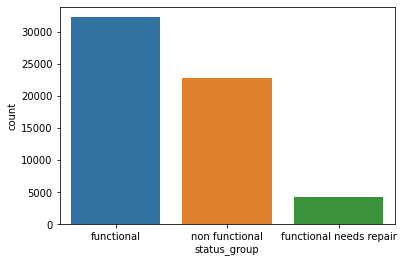
\includegraphics[scale=0.5]{figures/status_groups.png}
    \caption{Distribution of the target variable}
    \label{fig:status_groups}
\end{figure}

\section{Data Wrangling \& Pre-Processing}

The dataset requires some pre-processing and data wrangling to be performed. Firstly, there are some irrelevant features that need to be identified and dropped. The set of features to dropped will be continually modified and tested throughout the project.

Additionally, there are spelling mistakes in the "Funder" and "Installer" columns. This can be dealt with in two ways:
    \begin{itemize}
        \item (1) We can bin each value into a category, and then use the category as a feature. These categories will be for example: "Charity", "Government", "Religious", etc.
        \item (2) We can correct each spelling mistake to the correct value, and then bin any values with a value count smaller than a threshold into the "Other" category, keeping all other values.
    \end{itemize}

Both (1) and (2) will be tested throughout the project, and we will see which method works best. 


The missing values in the "Latitude", "Longitude" \& "Population" columns can be imputed using mean imputation, calculating the mean of the relevant area ("subvillage", "ward", ...). If there are still NaNs, we will increase the size of the 'area', up to "basin". For example, first we will impute the Population using the mean of the relevant subvillage, then if there are still NaNs, we will impute using the mean of the relevant ward. This process will repeat up to "basin".

The region column needs to be binned, and this can be done using data from the Tanzanian Water and Santitation Network, which already classifies each region into groups such as "Western Zone" or "Southern Highlands".

The dataset also contains a lot of categorical features, therefore, we must perform feature encoding before proceeding with feature selection and modelling. Basic label encoding will be used rather than one-hot encoding to avoid creating too many features which leads to curse of dimensionality. Finally, some feature engineering will be performed, such as creating a new feature that calculates the age of a well based on the constructed data and the date recorded.



\end{document}




